% Auto-generated by figures/src/make_captions.py (numbers from figures/src/data). Usage:
% \begin{figure}[t]\centering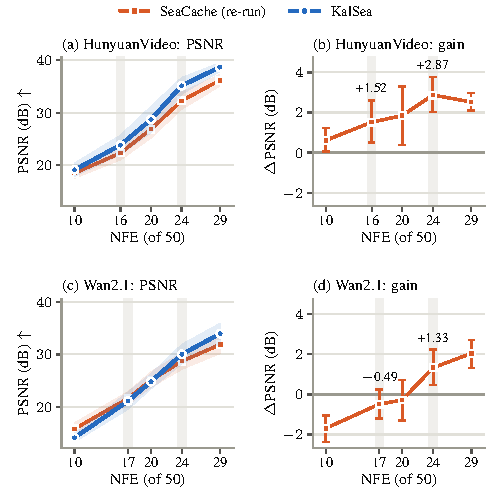
\includegraphics[width=\columnwidth]{figures/fig_video_sweep.pdf}% Auto-generated by figures/src/make_captions.py (numbers from figures/src/data). Usage:
% \begin{figure}[t]\centering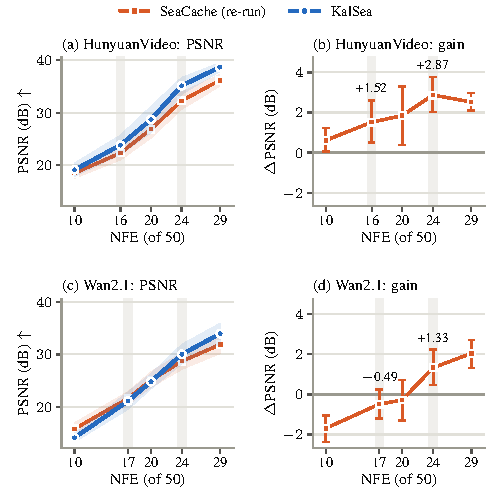
\includegraphics[width=\columnwidth]{figures/fig_video_sweep.pdf}% Auto-generated by figures/src/make_captions.py (numbers from figures/src/data). Usage:
% \begin{figure}[t]\centering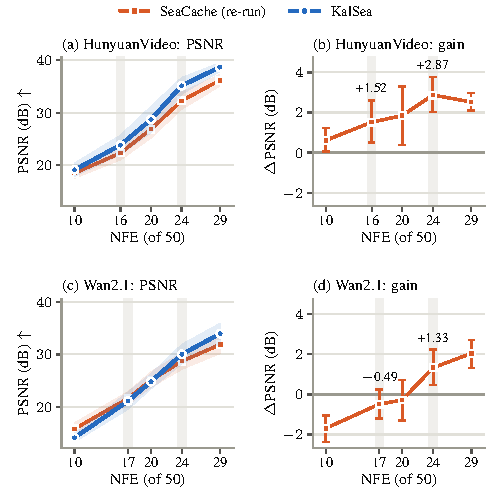
\includegraphics[width=\columnwidth]{figures/fig_video_sweep.pdf}% Auto-generated by figures/src/make_captions.py (numbers from figures/src/data). Usage:
% \begin{figure}[t]\centering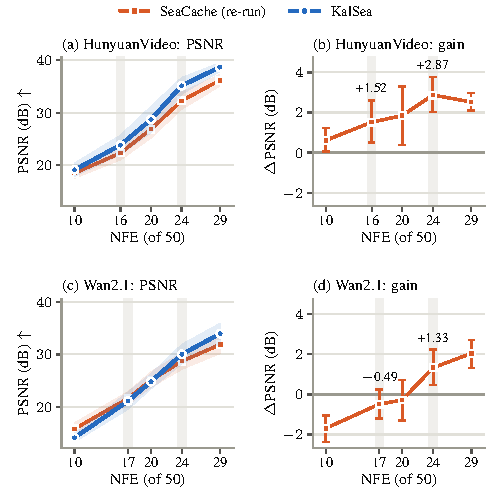
\includegraphics[width=\columnwidth]{figures/fig_video_sweep.pdf}\input{figures/fig_video_sweep_caption}\end{figure}   (supplement)
\caption{\textbf{Budget sweep on video} (20 VBench prompts per model, those of \cref{tab:supp-video-abl}; HunyuanVideo with the corrected gate). \textbf{(a, c)}~PSNR w.r.t.\ the 50-step reference vs.\ \nfe for our same-setup re-run of \seacache and for \ours, which share the \sea gate and its threshold (HunyuanVideo $\delta\in\{0.195, 0.2575, 0.35, 0.48, 0.865\}$, Wan2.1 $\delta\in\{0.14, 0.2, 0.265, 0.35, 0.815\}$); lines: means, shaded: 95\% bootstrap CIs. \textbf{(b, d)}~Paired PSNR gain of \ours over \seacache (mean, 95\% CI); gray bands: the budgets of the main paper's \maincref{tab:video-main}. On HunyuanVideo, \ours is better at every budget (+0.61\,dB [+0.05, +1.22] at 10 \nfe, +2.53\,dB [+2.11, +2.97] at 29). On Wan2.1 the gain shrinks with the budget: it is significant at 29 and 24 \nfe, not significant at 20 and 17 \nfe, and negative at 10 \nfe ($-$1.69\,dB [$-$2.37, $-$1.07]). Both methods computed the same steps on at least 19 (HunyuanVideo) and 15 (Wan2.1) of the 20 prompts at every threshold.}
\label{fig:video-sweep}
\end{figure}   (supplement)
\caption{\textbf{Budget sweep on video} (20 VBench prompts per model, those of \cref{tab:supp-video-abl}; HunyuanVideo with the corrected gate). \textbf{(a, c)}~PSNR w.r.t.\ the 50-step reference vs.\ \nfe for our same-setup re-run of \seacache and for \ours, which share the \sea gate and its threshold (HunyuanVideo $\delta\in\{0.195, 0.2575, 0.35, 0.48, 0.865\}$, Wan2.1 $\delta\in\{0.14, 0.2, 0.265, 0.35, 0.815\}$); lines: means, shaded: 95\% bootstrap CIs. \textbf{(b, d)}~Paired PSNR gain of \ours over \seacache (mean, 95\% CI); gray bands: the budgets of the main paper's \maincref{tab:video-main}. On HunyuanVideo, \ours is better at every budget (+0.61\,dB [+0.05, +1.22] at 10 \nfe, +2.53\,dB [+2.11, +2.97] at 29). On Wan2.1 the gain shrinks with the budget: it is significant at 29 and 24 \nfe, not significant at 20 and 17 \nfe, and negative at 10 \nfe ($-$1.69\,dB [$-$2.37, $-$1.07]). Both methods computed the same steps on at least 19 (HunyuanVideo) and 15 (Wan2.1) of the 20 prompts at every threshold.}
\label{fig:video-sweep}
\end{figure}   (supplement)
\caption{\textbf{Budget sweep on video} (20 VBench prompts per model, those of \cref{tab:supp-video-abl}; HunyuanVideo with the corrected gate). \textbf{(a, c)}~PSNR w.r.t.\ the 50-step reference vs.\ \nfe for our same-setup re-run of \seacache and for \ours, which share the \sea gate and its threshold (HunyuanVideo $\delta\in\{0.195, 0.2575, 0.35, 0.48, 0.865\}$, Wan2.1 $\delta\in\{0.14, 0.2, 0.265, 0.35, 0.815\}$); lines: means, shaded: 95\% bootstrap CIs. \textbf{(b, d)}~Paired PSNR gain of \ours over \seacache (mean, 95\% CI); gray bands: the budgets of the main paper's \maincref{tab:video-main}. On HunyuanVideo, \ours is better at every budget (+0.61\,dB [+0.05, +1.22] at 10 \nfe, +2.53\,dB [+2.11, +2.97] at 29). On Wan2.1 the gain shrinks with the budget: it is significant at 29 and 24 \nfe, not significant at 20 and 17 \nfe, and negative at 10 \nfe ($-$1.69\,dB [$-$2.37, $-$1.07]). Both methods computed the same steps on at least 19 (HunyuanVideo) and 15 (Wan2.1) of the 20 prompts at every threshold.}
\label{fig:video-sweep}
\end{figure}   (supplement)
\caption{\textbf{Budget sweep on video} (20 VBench prompts per model, those of \cref{tab:supp-video-abl}; HunyuanVideo with the corrected gate). \textbf{(a, c)}~PSNR w.r.t.\ the 50-step reference vs.\ \nfe for our same-setup re-run of \seacache and for \ours, which share the \sea gate and its threshold (HunyuanVideo $\delta\in\{0.195, 0.2575, 0.35, 0.48, 0.865\}$, Wan2.1 $\delta\in\{0.14, 0.2, 0.265, 0.35, 0.815\}$); lines: means, shaded: 95\% bootstrap CIs. \textbf{(b, d)}~Paired PSNR gain of \ours over \seacache (mean, 95\% CI); gray bands: the budgets of the main paper's \maincref{tab:video-main}. On HunyuanVideo, \ours is better at every budget (+0.61\,dB [+0.05, +1.22] at 10 \nfe, +2.53\,dB [+2.11, +2.97] at 29). On Wan2.1 the gain shrinks with the budget: it is significant at 29 and 24 \nfe, not significant at 20 and 17 \nfe, and negative at 10 \nfe ($-$1.69\,dB [$-$2.37, $-$1.07]). Both methods computed the same steps on at least 19 (HunyuanVideo) and 15 (Wan2.1) of the 20 prompts at every threshold.}
\label{fig:video-sweep}
